\documentclass{article}
        \usepackage[margin=1in]{geometry}
        \usepackage{algorithm}
        \usepackage{algorithmic}
        \usepackage{hyperref}
        \usepackage{amsmath,amsfonts,amssymb,amsthm,commath,dsfont}
        \usepackage{bm}
        \usepackage{cancel}
        \usepackage{enumitem}
        \usepackage{framed}
        \usepackage{xspace}
        \usepackage{microtype}
        \usepackage{float}
        \usepackage[round]{natbib}
        \usepackage{cleveref}
        \usepackage[dvipsnames]{xcolor}
        \usepackage{graphicx}
        \usepackage{listings}
        \usepackage[breakable]{tcolorbox}
        \tcbset{breakable}
        \usepackage{mathtools}
        \usepackage{autonum}
        \usepackage{comment}
        \usepackage{booktabs}
        \usepackage{enumitem}
        \usepackage{subcaption}

        \newlist{legal}{enumerate}{10}
        \setlist[legal]{label*=\arabic*.}
        
        \newcommand{\colbar}{\rule[-3mm]{.3mm}{1.5em}}
        \newcommand{\rowbar}{\rule[.5ex]{1.5em}{.3mm}}
        \newcommand{\francis}[1]{{\color{blue}#1}}
        \DeclareMathOperator{\rank}{rank}
        
        \newcommand{\yb}[1]{{\color{blue} #1}}

        % following loops. stolen from djhsu
        \def\ddefloop#1{\ifx\ddefloop#1\else\ddef{#1}\expandafter\ddefloop\fi}
        % \bbA, \bbB, ...
        \def\ddef#1{\expandafter\def\csname bb#1\endcsname{\ensuremath{\mathbb{#1}}}}
        \ddefloop ABCDEFGHIJKLMNOPQRSTUVWXYZ\ddefloop
        
        % \cA, \cB, ...
        \def\ddef#1{\expandafter\def\csname c#1\endcsname{\ensuremath{\mathcal{#1}}}}
        \ddefloop ABCDEFGHIJKLMNOPQRSTUVWXYZ\ddefloop
        
        % \vA, \vB, ..., \va, \vb, ...
        \def\ddef#1{\expandafter\def\csname v#1\endcsname{\ensuremath{\boldsymbol{#1}}}}
        \ddefloop ABCDEFGHIJKLMNOPQRSTUVWXYZabcdefghijklmnopqrstuvwxyz\ddefloop
        
        % \valpha, \vbeta, ...,  \vGamma, \vDelta, ...,
        \def\ddef#1{\expandafter\def\csname v#1\endcsname{\ensuremath{\boldsymbol{\csname #1\endcsname}}}}
        \ddefloop {alpha}{beta}{gamma}{delta}{epsilon}{varepsilon}{zeta}{eta}{theta}{vartheta}{iota}{kappa}{lambda}{mu}{nu}{xi}{pi}{varpi}{rho}{varrho}{sigma}{varsigma}{tau}{upsilon}{phi}{varphi}{chi}{psi}{omega}{Gamma}{Delta}{Theta}{Lambda}{Xi}{Pi}{Sigma}{varSigma}{Upsilon}{Phi}{Psi}{Omega}{ell}\ddefloop

        \newcommand\T{{\scriptscriptstyle\mathsf{T}}}
        \def\diag{\textup{diag}}
        \newcommand{\bx}{{\boldsymbol x}}
        \newcommand{\xup}[1]{x^{({#1})}}
        \newcommand{\yup}[1]{y^{({#1})}}
        \newcommand{\bxup}[1]{{\bx}^{({#1})}}
        \DeclareMathOperator*{\argmin}{arg\,min}
        \DeclareMathOperator*{\argmax}{arg\,max}

        \def\SPAN{\textup{span}}
        \def\tu{\textup{u}}
        \def\R{\mathbb{R}}
        \def\E{\mathbb{E}}
        \def\Z{\mathbb{Z}}
        \def\be{\bm{e}}
        \def\nf{\nabla f}
        \def\veps{\varepsilon}
        \def\cl{\textup{cl}}
        \def\inte{\textup{int}}
        \def\dom{\textup{dom}}
        \def\Rad{\textup{Rad}}
        \def\lsq{\ell_{\textup{sq}}}
        \def\hcR{\widehat{\cR}}
        \def\hcRl{\hcR_\ell}
        \def\cRl{\cR_\ell}
        \def\hcE{\widehat{\cE}}
        \def\cEl{\cE_\ell}
        \def\hcEl{\hcE_\ell}
        \def\eps{\epsilon}
        \def\1{\mathds{1}}
        \newcommand{\red}[1]{{\color{red} #1}}
        \newcommand{\blue}[1]{{\color{blue} #1}}
        \def\srelu{\sigma_{\textup{r}}}
        \def\vsrelu{\vec{\sigma_{\textup{r}}}}
        \def\vol{\textup{vol}}

        \newcommand{\ip}[2]{\left\langle #1, #2 \right \rangle}
        \newcommand{\mjt}[1]{{\color{blue}\emph\textbf{[M:}~#1~\textbf{]}}}
        \newcommand{\sahand}[1]{{\color{green}\emph\textbf{[Sah:}~#1~\textbf{]}}}

        \newtheorem{fact}{Fact}
        \newtheorem{lemma}{Lemma}
        \newtheorem{claim}{Claim}
        \newtheorem{proposition}{Proposition}
        \newtheorem{theorem}{Theorem}
        \newtheorem{corollary}{Corollary}
        \newtheorem{condition}{Condition}
        \theoremstyle{definition}
        \newtheorem{definition}{Definition}
        \theoremstyle{remark}
        \newtheorem{remark}{Remark}
        \newtheorem{example}{Example}

        \newcommand{\ms}[1]{\textcolor{red}{#1}}
        \newcommand{\ziyin}[1]{\textcolor{blue}{#1}}

        
        
        \newenvironment{Q}
        {%
          \clearpage
          \item
        }
        {%
          \phantom{s} %lol doesn't work
          \bigskip
          % \textbf{Solution.}
        }

        \title{CS 446 / ECE 449 --- Homework 2}
        \author{\emph{yiminc2}}
        \date{Version 1.0}

        \newif\ifshowsolutions      
        %\showsolutionstrue

\begin{document}
\maketitle

\noindent\textbf{Instructions.}
\begin{itemize}
	\item
	      Homework is due \textbf{Wednesday, October $1^{st}$, 11:59 a.m}; you have \textbf{3} late days in total for \textbf{all Homeworks}.

	\item
	      Everyone must submit \textbf{individually} at gradescope under \texttt{hw2} and \texttt{hw2code}.

	\item
	      The ``written'' submission at \texttt{hw2} \textbf{must be typed}, and submitted in
	      any format gradescope accepts (to be safe, submit a PDF).  You may use \LaTeX, markdown,
	      google docs, MS word, whatever you like; but it must be typed!

	\item
	      When submitting at \texttt{hw2}, gradescope will ask you to \textbf{mark out boxes
		      around each of your answers}; please do this precisely!

	\item
	      Please make sure your NetID is clear and large on the first page of the homework.

	\item
	      Your solution \textbf{must} be written in your own words.
	      Please see the course webpage for full \textbf{academic integrity} information.
	      You should cite any external reference you use.

	\item
	      We reserve the right to reduce the auto-graded score for
	      \texttt{hw2code} if we detect funny business (e.g., your solution
	      lacks any algorithm and hard-code answers you obtained from
	      someone else, or simply via trial-and-error with the autograder).

	\item
	      When submitting to \texttt{HW2 coding}, only upload \texttt{hw2\_q2.py}, \texttt{hw2\_q4.py} and \texttt{hw2\_utils.py}. Additional files will be ignored. (\textbf{DO NOT change the name of these three files!})

\end{itemize}
\begin{enumerate}[font={\Large\bfseries},left=0pt]
	\begin{Q}
		\textbf{\Large  Naive Bayes (25 pt)}

		\begin{enumerate}

			\item  In Naive Bayes classification, the number of parameters to be estimated for a Bayesian classifier is reduced by assuming conditional independence when modeling $P(X|Y)$. Conditional independence is defined as follows:

			      \textbf{Definition:} Let $X$, $Y$, and $Z$ be random variables. We say that $X$ is conditionally independent of $Y$ given $Z$, written as $X \perp Y | Z$, if and only if:


			      \[
				      P(X = x_i|Y = y_j, Z = z_k) = P(X = x_i|Z = z_k), \forall i, j, k
			      \]

			      Given this definition, please answer the following questions:

			      \begin{enumerate}
				      \item If $X \perp Y | Z$, can we conclude that
				            $P(X,Y | Z) = P(X | Z)P(Y | Z)$?
				            Explain your reasoning. (2 pt)

				      \item If $X \perp Y | Z$, can we conclude that
				            $P(X, Y) = P(X)P(Y)$?
				            Explain your reasoning. (2 pt)

				      \item Suppose $X$ is a vector of $d$ Boolean attributes, and $Y$ is a discrete variable that takes $C$ possible values. Let $\theta_{jc} = P(X_j | Y = c)$. How many independent $\theta_{jc}$ parameters must be estimated? (2 pt)

				      \item Now suppose $X$ is a vector of $d$ real-valued attributes, and each $X_j$ follows a Normal (Gaussian) distribution: $P(X_j = x_j | Y = c) = \mathcal{N}(x_j | \mu_{jc}, \sigma_{jc})$. How many distinct $\mu_{jc}$ and $\sigma_{jc}$ parameters must be estimated? (2 pt)\\

				      \item We can write the classification rule for Naive Bayes as:
				            \[
					            Y^{\text new} \leftarrow \arg\max_c \frac{P(Y = c)\prod_{j=1}^{d} P(X_j^{\text new}|Y = c)}{\sum_{v=1}^C P(Y = v)\prod_{k=1}^{d} P(X_k^{\text new}|Y = v)}
				            \]
				            When estimating $Y$, we often omit the denominator in the calculation. Why is it acceptable to do this? (2 pt)

				      \item Is it possible to compute $P(X)$ using the parameters estimated in Naive Bayes? (2 pt)

			      \end{enumerate}
			\item
			      Consider a classification problem where the input vector \( X = < X_1, X_2, X_3> \) consists of three boolean features \( X_j \in \{0,1\}, j = \{1,2,3\} \) and the label \( Y \in \{0,1\} \). You are given a dataset of \( N \) i.i.d. labeled examples \( \{X^{(i)},y^{(i)}\}_{i=1}^{N} \). For $X_1, X_2$ and $X_3$ we have:
			      $P(X_1 \vert X_2, X_3,Y) = P(X_1 | Y), ~P(X_2 \vert X_1, X_3, Y) = P(X_2 \vert Y)$ and $P(X_3 \vert X_1, X_2, Y) = P(X_3 \vert X_1)$.

			      \begin{enumerate}
				      \item
				            Express the joint distribution \( P(X_1, X_2, X_3, Y) \) as a product of simpler conditional probabilities, i.e. each variable depends only on atmost one another variable. (2 pt)

				      \item
				            Derive the maximum likelihood estimators for the following quantities (6 pt, 2pt each) :
				            \begin{enumerate}
					            \item \(  P(Y = 1) \)
					            \item \( P(X_1 = 1 \mid Y = y) \), for \( y \in \{0,1\} \).
					            \item \(  P(X_3 = 1 \mid Y = y) \), for $y \in \{0,1\}.$
				            \end{enumerate}

				            \textit{Note:}  It is sufficient to leave your answers as sums of indicator functions or fractions.

			      \end{enumerate}
			\item
			      Consider the same conditional independence structure as in Part~(b), but this time with continuous features $X_j$ drawn from Gaussian distributions instead of boolean. Specifically, let \(P(Y=0)=P(Y=1)=0.5\) and

			      \[
				      \begin{aligned}
					       & (X_1 \mid Y=y) \sim \mathcal N(\mu_{1y},1), \quad &  & \mu_{10}=0,\;\mu_{11}=1,                 \\
					       & (X_2 \mid Y=y) \sim \mathcal N(\mu_{2y},1), \quad &  & \mu_{20}=0,\;\mu_{21}=1,                 \\
					       & (X_3 \mid X_1=x_1) \sim \mathcal N(2x_1,1)\quad   &  & \text{(independent of $Y$ given $X_1$).}
				      \end{aligned}
			      \]
			      \begin{enumerate}
				      \item Derive the MAP rule for a new point $X^{\text{new}}$. (2 pt)
				      \item Using your classification rule, classify the following two points:
				            \[
					            X^{(a)} = <0.2, 0.7,-10>,
					            \qquad
					            X^{(b)} = <0.2, 0.7 ,10>.
				            \]
				            Do the predicted labels differ between these two cases? Explain why or why not. (3 pt)
			      \end{enumerate}


		\end{enumerate}

	\end{Q}
	\begin{tcolorbox}
		\begin{enumerate}
			\item \begin{enumerate}
				      \item \text{If $X \perp Y \mid Z$, \text{can we conclude that } $P(X, Y \mid Z) = P(X \mid Z)P(Y \mid Z)$?}  \\
				            \textbf{Ans: Yes} \\
				            \begin{align}
					            P(X, Y \mid Z) & = \frac{P(X, Y, Z)}{P(Z)}                                              \\
					                           & = \frac{P(Z)P(X, Y \mid Z)}{P(Z)}                                      \\
					                           & = \frac{P(Z)P(Y \mid Z)P(X \mid Y, Z)}{P(Z)} \quad \text{(chain rule)} \\
					                           & = \frac{P(Z)}P(Y \mid Z)P(X \mid Z){P(Z)} \quad (Y \perp X \mid Z)     \\
					                           & = P(Y \mid Z)P(X \mid Z)                                               \\
				            \end{align}

				      \item \text{If $X \perp Y \mid Z$, \text{can we conclude that } $P(X, Y \mid Z) = P(X \mid Z)P(Y \mid Z)$?}  \\
				            \textbf{Ans: No} \\
				            \begin{align}
					             & \because P(X, Y) = P(X)P(Y) \iff X \perp Y \text{, and we only know that } X \perp Y \mid Z \\
					             & \therefore P(X, Y) \neq P(X)P(Y)
				            \end{align}

				      \item How many independent $\theta_{jc}$ parameters must be estimated? \\
				            \textbf{Ans: C $\times$ d indepedent $\theta_{jc}$ parameters}
				            \begin{itemize}
					            \item $X$ has $d$ attributes.
					            \item For each class c, we estimate $\theta_{jc}$ for each attribute $X_j$.
					            \item Therefore, the total number of independent parameters is $C \times d$.
				            \end{itemize}

				      \item How many distinct $\mu_{jc}$ and $\sigma_{jc}$ parameters must be estimated? \\
				            \textbf{Ans: $2 \times C \times d$ distinct $\mu_{jc}$ and $\sigma_{jc}$ parameters with both having the same number $C \times d$}
				            \begin{itemize}
					            \item Each attribute $X_j$ requires a distinct set of $\mu_{jc}$ and $\sigma_{jc}$
					            \item The respective numbers of $\mu_{jc}$ and $\sigma_{jc}$ are both $C \times d$
					            \item Therefore, the total number of distinct parameters are $2 \times C \times d$
				            \end{itemize}

				      \item Why is omitting the denominator in the calculation acceptable for the estimation of Y. \\
				            \textbf{Ans: The $Y$ variable is not dependent on the denominator as the denominator is just a constant for normalization.}

				      \item Is it possible to calculate the $P(X)$ with Naive Bayes? \\
				            \textbf{Ans: Yes.} \\
				            \begin{itemize}
					            \item Given $P(X = x) = \sum^C_{c = 1} P(X = x \mid Y = c)P(Y = c) $
					            \item and the likelihood of Naive Bayes: $P(X \mid Y) = \prod^{d}_{j = 1} P(X_j \mid Y = c)$,
					            \item we can derive that $P(X) = \sum^C_{c = 1}P(Y = c) \prod^d_{j = 1} P(X_j \mid Y = c)$
				            \end{itemize}
			      \end{enumerate}


			\item \begin{enumerate}

				      \item Express the joint distribution $P(X_1, X_2, X_3, Y)$ as a product of simpler conditional probabilty. \\
				            \textbf{Ans: $P(Y)P(X_1 \mid Y)P(X_3)P(X_2 \mid Y)$}
				            \begin{itemize}
					            \item $P(X_1 \mid X_2, X_3, Y) = P(X_1 \mid Y) \Rightarrow X_1 \perp X_2, X_3 \mid Y$
					            \item $P(X_2 \mid X_1, X_3, Y) = P(X_2 \mid Y) \Rightarrow X_2 \perp X_1, X_3 \mid Y$
					            \item $P(X_3 \mid X_1, X_2, Y) = P(X_3 \mid X_1) \Rightarrow X_3 \perp X_2, Y \mid X_1$
				            \end{itemize}
				            \begin{align}
					            P(X_1, X_2, X_3, Y) & = P(Y)P(X_1, X_2, X_3 \mid Y)                                                                                                 \\
					                                & = P(Y)P(X_1 \mid Y)P(X_2, X_3 \mid X_1, Y)                                                                                    \\
					                                & = P(Y)P(X_1 \mid Y)\underbrace{P(X_3 \mid X_1, Y)}_{= P(X_3 \mid X_1)}\underbrace{P(X_2 \mid X_3,  X_1, Y)}_{= P(X_2 \mid Y)} \\
					                                & = P(Y)P(X_1 \mid Y)P(X_3 \mid X_1)P(X_2 \mid Y)                                                                               \\
				            \end{align}

				      \item Derive the maximum likelihood estimators for the following quantities: \\
				            Assume that $\mathbb{I}$ is the indicator function s.t. $\mathbb{I}\{e\} = \begin{cases}1 \quad (\text{e is true}) \\ 0 \quad (\text{e is wrong})\end{cases}$
				            \begin{enumerate}
					            \item P(Y = 1) \\
					                  \textbf{Ans: $\frac{\sum^{N}_{i = 1} \mathbb{I}\{y^{(i)} = 1\}}{N}$}
					            \item $P(X_1 = 1 \mid Y = y), \text{for } y \in \{0, 1\}$  \\
					                  \textbf{Ans: $\frac{\sum^{N}_{i = 1}\mathbb{I}\{x_1^{(i)} = 1, y^{(i)} = y\}}{\sum^{N}_{i = 1} \mathbb{I}\{y^{(i)} = y\}}$}
					            \item $P(X_3 = 1 \mid Y = y), \text{for } y \in \{0, 1\}$  \\
					                  \textbf{Ans: $\sum^{1}_{x_1 = 0} \frac{\sum^{N}_{i = 0} \mathbb{I}\{x^{(i)}_1 = x_1, x_3^{(i)} = 1\}}{\sum^{N}_{i = 0} \mathbb{I}\{x^{(i)}_1 = x_1\}} \frac{\sum^{N}_{i = 1} \mathbb{I}\{y^{(i)} = y, x^{(i)}_1 = x_1  \}}{\sum^{N}_{i = 1} \mathbb{I}\{y^{(i)} = y\}}$}

					                  \begin{align}
						                   & P(X_3 \mid Y) = \sum^{1}_{x_1 = 0} P(X_3, X_1 = x_1 \mid Y) \quad (Marginalization)                                                                                                                                                                                                          \\
						                   & P(X_3 \mid Y) = \sum^{1}_{x_1 = 0} P(X_3 \mid X_1 = x_1, Y) P(X_1 = x_1 \mid Y)                                                                                                                                                                                                              \\
						                   & \Rightarrow P(X_3 = 1 \mid Y = y) = \sum^{1}_{x_1 = 0} P(X_3 = 1 \mid X_1 = x_1)P(X_1 = x_1 \mid Y)                                                                                                                                                                                          \\
						                   & \Rightarrow P(X_3 = 1 \mid Y = y) = \sum^{1}_{x_1 = 0} \frac{\sum^{N}_{i = 0} \mathbb{I}\{x^{(i)}_1 = x_1, x_3^{(i)} = 1\}}{\sum^{N}_{i = 0} \mathbb{I}\{x^{(i)}_1 = x_1\}} \frac{\sum^{N}_{i = 1} \mathbb{I}\{y^{(i)} = y, x^{(i)}_1 = x_1  \}}{\sum^{N}_{i = 1} \mathbb{I}\{y^{(i)} = y\}}
					                  \end{align}

				            \end{enumerate}
			      \end{enumerate}
			\item \begin{enumerate}
				      \item Derive the MAP for a new point $X^{new}$ \\
				            \textbf{Ans: } $\begin{cases} 1 \quad (x_1 + x_2 > 1) \\ 0 \quad(otherwise) \end{cases}$ \\
				            Given the same conditional independence structure
				            \begin{align}
					             & P(X_1, X_2, X_3, Y) = P(Y)P(X_1 \mid Y)P(X_2 \mid Y)P(X_3 \mid X_1)                     \\
					             & \Rightarrow P(X_1, X_2, X_3 \mid Y)P(Y) = P(Y)P(X_1 \mid Y)P(X_2 \mid Y)P(X_3 \mid X_1) \\
					             & \Rightarrow P(X_1, X_2, X_3 \mid Y) = P(X_1 \mid Y)P(X_2 \mid Y)P(X_3 \mid X_1)
				            \end{align}

				            Under the condition where Y = 1 is chosen:

				            \begin{align}
					             & P(Y=1 \mid X_1,X_2,X_3) > P(Y=0 \mid X_1,X_2,X_3)                                                                                \\
					             & \iff P(Y=1)\,P(X_1,X_2,X_3 \mid Y=1) > P(Y=0)\,P(X_1,X_2,X_3 \mid Y=0)                                                           \\
					             & \iff P(X_1\mid Y=1)P(X_2\mid Y=1) > P(X_1\mid Y=0)P(X_2\mid Y=0)                                                                 \\
					             & \iff \log\frac{P(X_1\mid Y=1)}{P(X_1\mid Y=0)} + \log\frac{P(X_2\mid Y=1)}{P(X_2\mid Y=0)} > 0                                   \\
					             & \iff -\tfrac12\!\left[(x_1-\mu_{11})^2 - (x_1-\mu_{10})^2\right] -\tfrac12\!\left[(x_2-\mu_{21})^2 - (x_2-\mu_{20})^2\right] > 0 \\
					             & \iff (\mu_{11}-\mu_{10})x_1 - \tfrac12(\mu_{11}^2-\mu_{10}^2) + (\mu_{21}-\mu_{20})x_2 - \tfrac12(\mu_{21}^2-\mu_{20}^2) > 0
				            \end{align}

				            Plug the values of $\mu$s in

				            \begin{align}
					             & x_1 - \tfrac12 + x_2 - \tfrac12 > 0
					             & x_1 + x_2 > 1
				            \end{align}

				            Therefore, the MAP for a new point $X^{new}$ is

				            $$
					            \begin{cases}
						            1 \quad (x_1 + x_2 > 1) \\
						            0 \quad(otherwise)
					            \end{cases}
				            $$


				      \item Using your classification rule, classify the following two points:
				            $$
					            X^{(a)} = <0.2, 0.7, -10>, \quad\quad X^{(b)} = <0.2, 0.7, 10>
				            $$
				            Do the predicted labels differ between these two cases? Explain why? \\
				            \textbf{Ans: Both $X^{(a)}$ and $X^{(b)}$ are classified with the label $y = 0$ as the sum of their $X_1$ and $X_2$ are equal ($0.9$) and their $X_3$ values are not used by the classifier.}

			      \end{enumerate}

		\end{enumerate}
	\end{tcolorbox}
	\begin{Q}
		\textbf{\Large  Gaussian Naive Bayes. (25 pt)}

		Recall from Lecture 7 (slide 5), taking $\log(\cdot)$ of the objective function, we have the decision rule as :

		$$
			Y^{\text{new}} = \argmax_y \left( \biggl(\, \sum_{j=1}^d \log P(X_j^{\text{new}} | Y = y) \biggr) +\log P(Y=y) \right)
		$$

		In a Gaussian Naive Bayes, the features $X^{\text{new}}_j$ are continuous variables, and the probability $P(X^{\text{new}}_j|Y=y)$ is modeled as a Gaussian distribution

		$$
			P(X^{\text{new}}_j|Y=y)= \mathcal{N}(X^{\text{new}}_j\mid\mu_{y,j},\sigma^2_{y,j})
		$$

		For simplicity, we assume that there exists at least example that belong to each class.
		\begin{itemize}
			\item There are $d$ attributes to describe each example.
			\item We use pair $(\bm{x}^{(i)},y^{(i)})$ to represent $i$th example, where $\bm{x}^{(i)}$ is a length-$d$ vector that describes its properties, and $y^{(i)}$ is a scalar representing its label.
			\item For $j\in\{1,2,\cdots,d\}$, $x^{(i)}_j\in \mathbb{R}$ is the value of attribute $j$ of each example $i$; $y^{(i)}=0$ means example $i$ is in class $0$, and $y^{(i)}=1$ means example $i$ is in class $1$.
			\item We use $(\bm{X},\bm{y})$ to represent a dataset of size $N$, where $\bm{X}=\left(\bx^{(1)}, \bx^{(2)},\cdots,\bx^{(N)}\right)^\top$ is a $N\times d$ matrix, and $\bm{y}=\left(y^{(1)},y^{(2)},\cdots,y^{(N)}\right)$ is a length-$N$ vector.
		\end{itemize}

		You are given two datasets in this homework: $(\bm{X}_\mathrm{train},\bm{y}_\mathrm{train})$ and $(\bm{X}_\mathrm{test},\bm{y}_\mathrm{test})$, which can be obtained by calling \texttt{gaussian\_dataset("train")} and \texttt{gaussian\_dataset("test")} in \texttt{hw2\_utils.py}. Your tasks are:

		\begin{enumerate}

			\item Implement the function \texttt{gaussian\_theta(X, y)} in \texttt{hw2\_q2.py}.

			      The input is the training dataset $(\bm{X}_\mathrm{train},\bm{y}_\mathrm{train})$. The output is $(\bm{\mu}, \bm{\sigma}^2)$. Both of them are $2\times d$ matrices in PyTorch float tensor, where $\mu_{y,j}$ and $\sigma_{y,j}^2$ are Gaussian distribution parameters of the MLE estimation of $P(X_j=1\mid Y=y)$. (8 pt)


			\item Implement the function \texttt{gaussian\_p(y)} in \texttt{hw2\_q2.py}.

			      The input is the label part $\bm{y}_\mathrm{train}$ of the training dataset. The output $p$ is a scalar, which is the MLE for $P(Y=0)$. (4 pt)

			\item Implement the function \texttt{gaussian\_classify(mu, sigma2, p, X)} in \texttt{hw2\_q2.py}.

			      The input is the output $\bm{\mu},\bm{\sigma^2},p$ from the two functions above, and the label part $\bm{X}_\mathrm{test}$ of the testing dataset of size $N$. The output $\bm{\widehat{y}}$ is an length-$N$ vector, where $\bm{\widehat{y}}^{(i)}$ is the predicted label (0 or 1) for the object with properties $\bm{x}^{(i)}_\mathrm{test}$, or the $i$-th row of $\bm{X}_\mathrm{test}$. For simplicity, it's guaranteed that there will be no ties (so the $\argmax$ will be unique). (6pt)

			      \textbf{Note:} Please use the logarithmic form of both $\widehat{Y}$ and Gaussian  PDF  to avoid precision issues.

			      \textbf{Library routines:} \texttt{torch.log}, \texttt{torch.sum}, \texttt{torch.mean}, \texttt{torch.var} (Please use \texttt{unbiased=False}).
			\item
			      Show that, in Gaussian Naive Bayes with equal class priors $P(Y=0)=P(Y=1)=0.5$ and
			      with class-conditional distributions
			      \[
				      (X_j \mid Y=y) \;\sim\; \mathcal N(\mu_{y,j}, \sigma_j^2),
			      \]
			      where the variances $\sigma_j^2$ are the same across classes (but may differ across features),
			      the MAP classification rule is equivalent to a \emph{linear classifier} in $\bx=< x_1,\dots,x_d >$.
			      That is, derive the explicit form of the decision boundary and show it can be written as
			      \[
				      \widehat{ y}(\bx) =
				      \begin{cases}
					      1, & \text{if } \sum_{j=1}^d w_j x_j > \tau, \\
					      0, & \text{if } \sum_{j=1}^d w_j x_j < \tau.
				      \end{cases}
			      \]
			      for some weights $w_j$ and threshold $\tau$ depending on $(\mu_{0,j},\mu_{1,j},\sigma_j^2)$. (7pt)

		\end{enumerate}



	\end{Q}
	\begin{tcolorbox}
		(d) To label input data with 1, $P(Y = 1 \mid X_j) > P(Y = 0 \mid X_j)$ should hold.

		\begin{align}
			 & P(Y=1 \mid x) > P(Y=0 \mid x)                                                                                                            \\
			 & \iff P(x \mid Y=1) > P(x \mid Y=0) \qquad (\text{equal priors})                                                                          \\
			 & \iff \prod_{j=1}^d P(X_j=x_j \mid Y=1) > \prod_{j=1}^d P(X_j=x_j \mid Y=0)                                                               \\
			 & \iff \sum_{j=1}^d \log P(X_j=x_j \mid Y=1) > \sum_{j=1}^d \log P(X_j=x_j \mid Y=0)                                                       \\
			 & \iff \sum_{j=1}^d \left[
				-\tfrac12 \log(2\pi\sigma_j^2) - \frac{(x_j-\mu_{1j})^2}{2\sigma_j^2}
				\right]
			>
			\sum_{j=1}^d \left[
				-\tfrac12 \log(2\pi\sigma_j^2) - \frac{(x_j-\mu_{0j})^2}{2\sigma_j^2}
			\right]                                                                                                                                     \\
			 & \iff \sum_{j=1}^d \frac{(x_j-\mu_{0j})^2 - (x_j-\mu_{1j})^2}{2\sigma_j^2} > 0                                                            \\
			 & \iff \sum_{j=1}^d \frac{2x_j(\mu_{1j}-\mu_{0j}) + (\mu_{0j}^2-\mu_{1j}^2)}{2\sigma_j^2} > 0                                              \\
			 & \iff \sum_{j=1}^d \left(\frac{\mu_{1j}-\mu_{0j}}{\sigma_j^2}\right) x_j > - \frac{\mu_{0j}^2 - \mu_{1j}^2}{2\sigma^2_j}                  \\
			 & \text{Let } w_j = \left(\frac{\mu_{1j}-\mu_{0j}}{\sigma_j^2}\right)\text{, } \tau =- \frac{\mu_{0j}^2 - \mu_{1j}^2}{2\sigma^2_j}         \\
			 & \iff \sum^{d}_{j = 1} w_j x_j > \tau                                                                                                     \\
			 & \because P(Y = 1 \mid x) > P(Y = 0 \mid x) \iff \sum^{d}_{j = 1} w_j x_j > \tau\text{, and following the same proceudre, }               \\
			 & \text{we can derive }P(Y = 0 \mid x)> P(Y = 1 \mid x) \iff \sum^{d}_{j = 1} w_j x_j < \tau                                               \\
			 & \therefore \hat{y}(x) = \begin{cases} 1 \quad (\sum^{d}_{j = 1} w_j x_j > \tau) \\ 0 \quad (\sum^{d}_{j = 1} w_j x_j < \tau) \end{cases}
		\end{align}

	\end{tcolorbox}
	\begin{Q}
		\textbf{\Large Logistic Regression. (25 pt)}

		In logistic regression, the class probability is modeled as
		$$P(y^{(i)}|{\bf{x}}^{(i)}, {\bf{w}}) = \sigma(y^{(i)} {\bf{w}}^\top {\bf{x}}^{(i)})$$
		where ${\bf{x}}^{(i)} \in \mathbb{R}^{d+1}$ represents the feature vector, $y^{(i)} \in \{-1,+1\}$ is the class label, and $\sigma(s) = \frac{1}{1 + e^{-s}}$ is the sigmoid function.

		(Note: We exclude the bias term $w_0$ as it can be absorbed into the weight vector: ${\bf w}=\begin{bmatrix}\uparrow \\\bm w\\\downarrow \\ w_0\end{bmatrix}$, and transform $\bm x$ to ${\bf x}=\begin{bmatrix}\uparrow \\\bm x\\\downarrow \\ 1\end{bmatrix}$, which we discussed in Lecture 3 ``notation hack".)


		\begin{enumerate}
			\item Prove that the sigmoid function $\sigma(\cdot)$ satisfies the property
			      $$\sigma(-s) = 1 - \sigma(s)$$
			      By demonstrating this, show that, $P(y^{(i)} = -1 | \bm{x}^{(i)}) + P(y^{(i)} = 1 | \bm{x}^{(i)}) = 1$. (2 pt)

			\item Prove that
			      $$\sigma'(s) = \sigma(s)(1 - \sigma(s))$$  (2 pt)

			\item Derive the gradient of the log-likelihood function, that is, compute
			      $$\nabla_w \log P(\bm{y} | {\bf{X}}, \bf{w})$$
			      where $\bm{y} = [y^{(1)}, y^{(2)}, ..., y^{(N)}]^T$ and ${\bf{X}} = \{{\bf{x}}^{(1)}, {\bf{x}}^{(2)}, ..., {\bf{x}}^{(N)}\}$. (5 pt)

			\item Derive the Hessian matrix $\bm{H}$ of the log-likelihood function, where each entry $H_{ab}$ is given by
			      $$H_{ab} = \frac{\partial^2}{\partial w_a \partial w_b} \log P(\bm{y} | {\bf{X}}, \bf{w})$$  (5 pt)

			\item Prove that the Hessian is negative semi-definite, i.e., show that $\bm{z}^T \bm{H} \bm{z} \leq 0$ for any vector $\bm{z} \in \mathbb{R}^{d+1}$. By doing so, we can conclude that the log-likelihood is concave and has no local maxima, only a global maximum.   (5 pt)
			\item \textbf{Gradient Descent Update Rule:} Use the gradient of the log-likelihood to derive the weight update rule for one iteration of gradient descent. Assume a learning rate $\alpha$.  (3 pt)

			\item \textbf{Newton’s Method Update Rule:} Use Newton’s method incorporating the Hessian matrix to derive the weight update rule.  (3 pt)

		\end{enumerate}
	\end{Q}
	\begin{tcolorbox}
		\begin{enumerate}
			\item Prove that the sigmoid function satisfies the property $\sigma(-s) = 1 - \sigma(s)$,
			      and show that $P(y^{(i)} = -1 \mid x^{(i)}) + P(y^{(i)} = 1 \mid x^{(i)}) = 1$.

			      \begin{align}
				      \sigma(-s) & = \frac{1}{1 + e^s}                             \\
				                 & = \frac{1 + e^s}{1 + e^s} - \frac{e^s}{1 + e^s} \\
				                 & = 1 - \frac{e^s}{1 + e^s}                       \\
				                 & = 1 - \frac{1}{\frac{1}{e^s} + 1}               \\
				                 & = 1 - \frac{1}{e^{-s} + 1}                      \\
				                 & = 1 - \sigma(s)                                 \\
			      \end{align}

			      Given this proof we can derive that:

			      \begin{align}
				       & P(y^{(i)} = -1 \mid x^{(i)}) + P(y^{(i)} = 1 \mid x^{(i)})                                                                      \\
				       & = \sigma(-w^\intercal x^{(i)}) + \sigma{(w^\intercal x^{(i)})}                                                                  \\
				       & \because \sigma(-s) = 1 - \sigma(s)                                                                                             \\
				       & \therefore \sigma(-w^\intercal x^{(i)}) + \sigma{(w^\intercal x^{(i)})} = 1 - \sigma(w^\intercal x) + \sigma(w^\intercal x) = 1
			      \end{align}

			\item Prove that $\sigma'(s) = \sigma(s)(1 - \sigma(s))$

			      \begin{align}
				      \sigma'(s) & = -(1 + e^{-s})^{-2} (-e^{-s})                                          \\
				                 & = (1 + e^{-s})^{-1} (1 + e^{-s})^{-1}(e^{-s})                           \\
				                 & = \sigma(s) \frac{e^{-s}}{1 + e^{-s}}                                   \\
				                 & = \sigma(s) \underbrace{\frac{1}{e^s + 1}}_{\sigma(-s) = 1 - \sigma(s)} \\
				                 & = \sigma(s)(1 - \sigma(s))                                              \\
			      \end{align}

			\item Derive the gradient of the log-likelihood function. \\
			      \textbf{Ans: $X(\sigma(-y\odot Xw) \odot y)$}
			      \begin{align}
				      \log P(y \mid X, w)          & = \sum^{N}_{i = 1} \log P(y^{(i)} \mid x^{(i)}, w)                        \\
				                                   & = \sum^{N}_{i = 1} \log \sigma(y^{(i)}w^\intercal x^{(i)})                \\
				      \nabla_w \log P(y \mid X, w) & = \sum^{N}_{i = 1} (1 - \sigma(y^{(i)}w^\intercal x^{(i)}))y^{(i)}x^{(i)} \\
				                                   & = \sum^{N}_{i = 1} \sigma(- y^{(i)}w^\intercal x^{(i)})y^{(i)}x^{(i)}
			      \end{align}

			      Given $y = \left[y^{(1)}, y^{(2)}, \dots, y^{(N)}\right]^\intercal$ and  $X = \left[x^{(1)}, x^{(2)}, \dots, x^{(N)}\right]$, we rewrite the gradient in the matrix form:

			      \begin{align}
				       & \sum^{N}_{i = 1} \sigma(- y^{(i)}w^\intercal x^{(i)})y^{(i)}x^{(i)}                                                                        \\
				       & = X(\sigma(-y\odot Xw) \odot y) \quad\quad (Xc = \sum^N_{i = 1} c_i x^{(i)}\text{ where } c = \left[c_1, c_2, \dots, c_N\right]^\intercal)
			      \end{align}

			\item Derive the Hessian matrix H of the log-likelihood function. \\
			      \textbf{Ans: $-X D X^\intercal$} \\
			      Partially differentiate the previous result by w again

			      \begin{align}
				       & \frac{\partial}{\partial w} \sum^{N}_{i = 1} \sigma(- y^{(i)}w^\intercal x^{(i)})y^{(i)}x^{(i)}                                                   \\
				       & = \sum^{N}_{i = 1} \sigma(- y^{(i)}w^\intercal x^{(i)})(1 - \sigma(- y^{(i)}w^\intercal x^{(i)}))(-y^{(i)}x^{(i)})(y^{(i)}x^{(i)})                \\
				       & = \sum^{N}_{i = 1} (1 - \sigma(y^{(i)}w^\intercal x^{(i)}))\sigma(y^{(i)}w^\intercal x^{(i)})(-y^{(i)}x^{(i)})(y^{(i)}x^{(i)})                    \\
				       & = \sum^{N}_{i = 1} (1 - \sigma(y^{(i)}w^\intercal x^{(i)}))\sigma(y^{(i)}w^\intercal x^{(i)})(-x^{(i)})x^{(i)\intercal}   \quad (y \in \{1, -1\}) \\
			      \end{align}

			      Rewrite it into the matrix form

			      \begin{align}
				       & \sum^{N}_{i = 1} (1 - \sigma(y^{(i)}w^\intercal x^{(i)}))\sigma(y^{(i)}w^\intercal x^{(i)})(-x^{(i)})x^{(i)\intercal}                                       \\
				       & = -X \sum^{N}_{i = 1} (1 - \sigma(y^{(i)}w^\intercal x^{(i)}))\sigma(y^{(i)}w^\intercal x^{(i)})X^\intercal                                                 \\
				       & \because (1 - \sigma(y^{(i)}w^\intercal x^{(i)}))\sigma(y^{(i)}w^\intercal x^{(i)}) \text{ produces scalar values}                                          \\
				       & \therefore \text{we can rewrite} \sum^{N}_{i = 1} (1 - \sigma(y^{(i)}w^\intercal x^{(i)}))\sigma(y^{(i)}w^\intercal x^{(i)}) \text{as a diagonal matrix } D \\
				       & = -X D X^\intercal
			      \end{align}

			\item Prove that the Hessian is negative semi-definite.

			      \begin{align}
				      z^\intercal H z & = -z^\intercal X D X^\intercal z                                                                                                                          \\
				                      & = -(X^\intercal z)^\intercal D(X^\intercal z)                                                                                                             \\
				                      & \text{Let } a = X^\intercal z \text{, and rewrite the expression in quardratic form}                                                                      \\
				                      & = -\sum^{N}_{i = 1} (1 - \sigma(y^{(i)}w^\intercal x^{(i)}))\sigma(y^{(i)}w^\intercal x^{(i)}) a_i^2                                                      \\
				                      & \because (1 - \sigma(y^{(i)}w^\intercal x^{(i)}))\sigma(y^{(i)}w^\intercal x^{(i)}) \text{ and }a_i^2 \text{ should always be greater than or equal to 0} \\
				                      & \therefore -\sum^{N}_{i = 1} (1 - \sigma(y^{(i)}w^\intercal x^{(i)}))\sigma(y^{(i)}w^\intercal x^{(i)}) a_i^2 \le 0                                       \\
				                      & \therefore z^\intercal Hz\text{ is negative semi-definite}                                                                                                \\
			      \end{align}

			\item Use the gradient of the log-likelihood to derive the weight update rule for one iteration of gradient descent. \\
			      \textbf{Ans: $w_{t + 1}$ = $w_{t} + \alpha X(\sigma(-y\odot Xw) \odot y)$ at iteration $t$}

			\item Use Newton's method incoporating the Hessian matrix to derive the weight update rule.
			      \textbf{Ans: $w_{t+1} = w_{t} + (XDX^\intercal)^{-1} \nabla l(w_t)$}

			      To maximize the log-likelihood, we want want to achieve $\nabla l(w) = 0$. We approximate $l(w)$ with Taylor's expansion of gradient.
			      Namely, at iteration t, we have the update rule:

			      \begin{align}
				       & \nabla l(w_{t+1}) \approx \nabla l(w_{t}) + \nabla^2 l(w_t)(w_{t+1} - w_t) \\
			      \end{align}

			      To find the w such that $\nabla l(w) = 0$, we set the approximation to 0:

			      \begin{align}
				       & 0 \approx \nabla l(w_{t}) + \nabla^2 l(w_t)(w_{t+1} - w_t)                              \\
				       & \text{Let } g = \nabla l(w_t), \;\; H = \nabla^2 l(w_t),\;\; \Delta = (w_{t + 1} - w_t) \\
				       & \Rightarrow -g \approx H\Delta                                                          \\
				       & \Rightarrow -H^{-1}g \approx \Delta                                                     \\
			      \end{align}

			      Therefore, we can derive the Newton's Method update rule with our derived Hessian Matrix:

			      \begin{align}
				      w_{t + 1} & = w_t-H^{-1}g                                 \\
				                & = w_{t} - (-XDX^\intercal)^{-1} \nabla l(w_t) \\
				                & = w_{t} + (XDX^\intercal)^{-1} \nabla l(w_t)  \\
			      \end{align}



		\end{enumerate}
	\end{tcolorbox}
	\begin{Q}
		\textbf{\Large Programming - Optimization. (25 pt)}

		This assignment guides you through building, refining, and optimizing a Logistic Regression model from scratch. Complete the \texttt{TODO} sections in the provided Python code. You can either use the Jupyter Notebook (hw2\_q4.ipynb) or the Python file (hw2\_q4.py).

		\textbf{Submission Requirements}: If you use the Jupyter notebook, please make sure to convert it to hw2\_q4.py and submit it to Gradescope along with hw2\_q2.py and hw2\_utils.py. Submit all generated plots and write the discussion sections (4(a)iii, 4(b)ii, 4(d)ii) with your written assignment.

		\begin{enumerate}
			\item{Logistic Regression
			      \begin{enumerate}
				      \item Start by implementing the core components of a logistic regression model. (4 pt)
				            \begin{enumerate}
					            \item Implement the \textbf{sigmoid function}.
					            \item Implement the \textbf{cost function} (binary cross-entropy).  A cost function measures the total error between a model's predictions and the actual labels, summarizing its performance into a single number to be minimized. Binary cross-entropy (or Log Loss) is a specific cost function for binary classification that heavily penalizes predictions that are both confident and incorrect. Please see code for more information on how to implement this.
					            \item Compute the \textbf{gradients} for the weights and bias.
					            \item Implement the \textbf{parameter update rule} for gradient descent.
				            \end{enumerate}
				      \item \textbf{Feature Transformation:} Create new features from the existing ones using non-linear transforms (e.g., $x_1^2, x_2^2, x_1x_2$) to map the data into a higher-dimensional space. (4 pt)
				      \item \textbf{Discussion:} Analyze the generated plot of the decision boundary and explain why the model with transformed features can now correctly separate the data, whereas a linear model in the original feature space could not. (2 pt)
			      \end{enumerate}
			      }
			\item{L1 vs. L2 Regularization
			      \begin{enumerate}
				      \item For the same model, modify the cost function and gradient update steps to include options for L1 and L2 regularization. Note that L1 regularization (Lasso) adds a penalty equal to the sum of the absolute values of the weights. In contrast, L2 regularization (Ridge) adds a penalty equal to the sum of the squares of the weights. (4 pt)
				      \item \textbf{Discussion:} Train three separate models: one with L1 regularization, one with L2 regularization, and one with no regularization. Generate a plot that compares their decision boundaries. Compare the effects of L1 and L2 regularization on the model. What kind of effect does regularization have on the model weights? What is the main difference in how they affect the model's weights? When would you choose one over the other? (2 pt)
			      \end{enumerate}
			      }
			\item{Hyperparameter Tuning (2 pt)
			      \begin{enumerate}
				      \item This exercise will guide you through performing a grid search to tune the learning rate (\texttt{alpha}) and the L2 regularization (\texttt{lambda}) hyperparameters.
				            \begin{enumerate}
					            \item Define a set of \texttt{alpha} values and \texttt{lambda} values to test.
					            \item Train a model for each combination of \texttt{alpha} and \texttt{lambda}, and evaluate its performance on the validation set.
				            \end{enumerate}
				      \item Identify the best-performing hyperparameter combination. Train a final model on the full training set using these optimal values and generate a plot of its decision boundary.
			      \end{enumerate}
			      }
			\item{Gradient Descent Variants
			      \begin{enumerate}
				      \item Run through the implementation of Batch Gradient Descent, Mini-batch Gradient Descent, and Stochastic Gradient Descent. (6 pt)
				            \begin{enumerate}
					            \item \textbf{Batch Gradient Descent} uses the entire dataset to compute gradients in each step.
					            \item \textbf{Mini-batch Gradient Descent} processes data in small batches (e.g., size 32). In each step, you will compute the gradient and update the parameters based on just one mini-batch.
					            \item \textbf{Stochastic Gradient Descent (SGD)} updates the parameters after processing each single training example (i.e., a mini-batch of size 1).
				            \end{enumerate}
				      \item \textbf{Discussion:} Analyze the generated plot that visualizes the cost function over the number of updates for all three gradient descent variants. Discuss the trade-offs between the three methods. Compare them in terms of computational efficiency (speed) and stability of convergence. (1 pt)
			      \end{enumerate}
			      }
		\end{enumerate}
	\end{Q}
	\begin{tcolorbox}
		\begin{enumerate}
			\item iii. Given that the input data are in circular distribution which is linearly inseparable, the Logistic Regression model, a linear model, cannot classify the input data with a linear decision boundary (shown in Figure 1).

			      \begin{center}
				      \centering
				      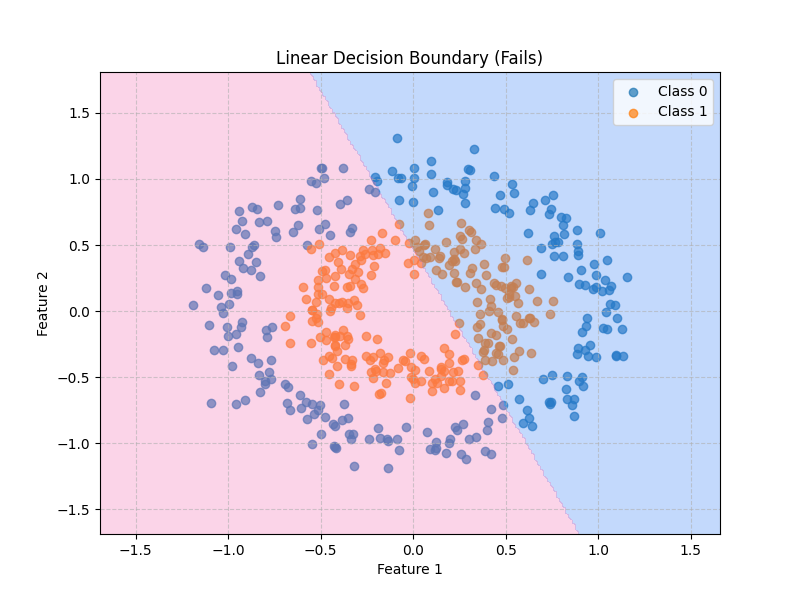
\includegraphics[width=0.7\linewidth]{submission_4a_linear_decision_boundary.png} \\
				      \textbf{Figure 1:} Linear Decision Boundary
			      \end{center}

			      However, by mapping the existing data points to higher dimensions, we enable our linear model to capture the non-linear patterns in the data (shown in Figure 2).

			      \begin{center}
				      \centering
				      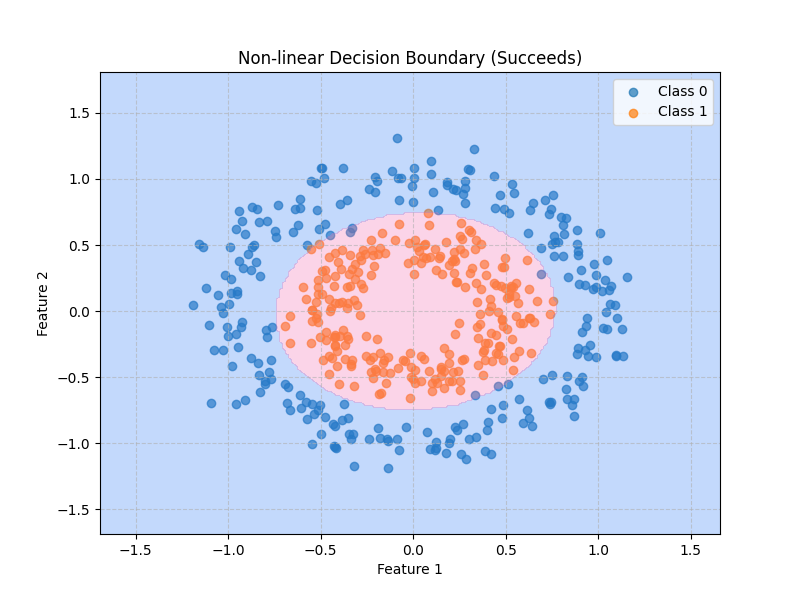
\includegraphics[width=0.7\linewidth]{submission_4a_nonlinear_decision_boundary.png} \\
				      \textbf{Figure 2:} Non-linear Decision Boundary
			      \end{center}
			\item ii. As shown in Figure 3, both L1 and L2 regularizations bring down the weights when they are large, which suppresses the overfitting problem for the model.
			      Both regularizations penalize large weights by introducing penalty terms ($L1: \frac{\lambda}{m}\mid\mid w\mid\mid_1,\quad L2: \frac{\lambda}{2m}\mid\mid w\mid\mid_2^2$).
			      The difference is that while L2 regularization shrinks weights proportially to their current values (gradient penalty: $\lambda w$) during gradient descent, the L1 regularization pulls the insignificant features to zero (gradient penalty: $\lambda$).
			      Therefore, L1 regularization should be adopted where only certain features matter; whereas, L2 regularization should be considered when all features need to be preserved.

			      \begin{center}
				      \centering
				      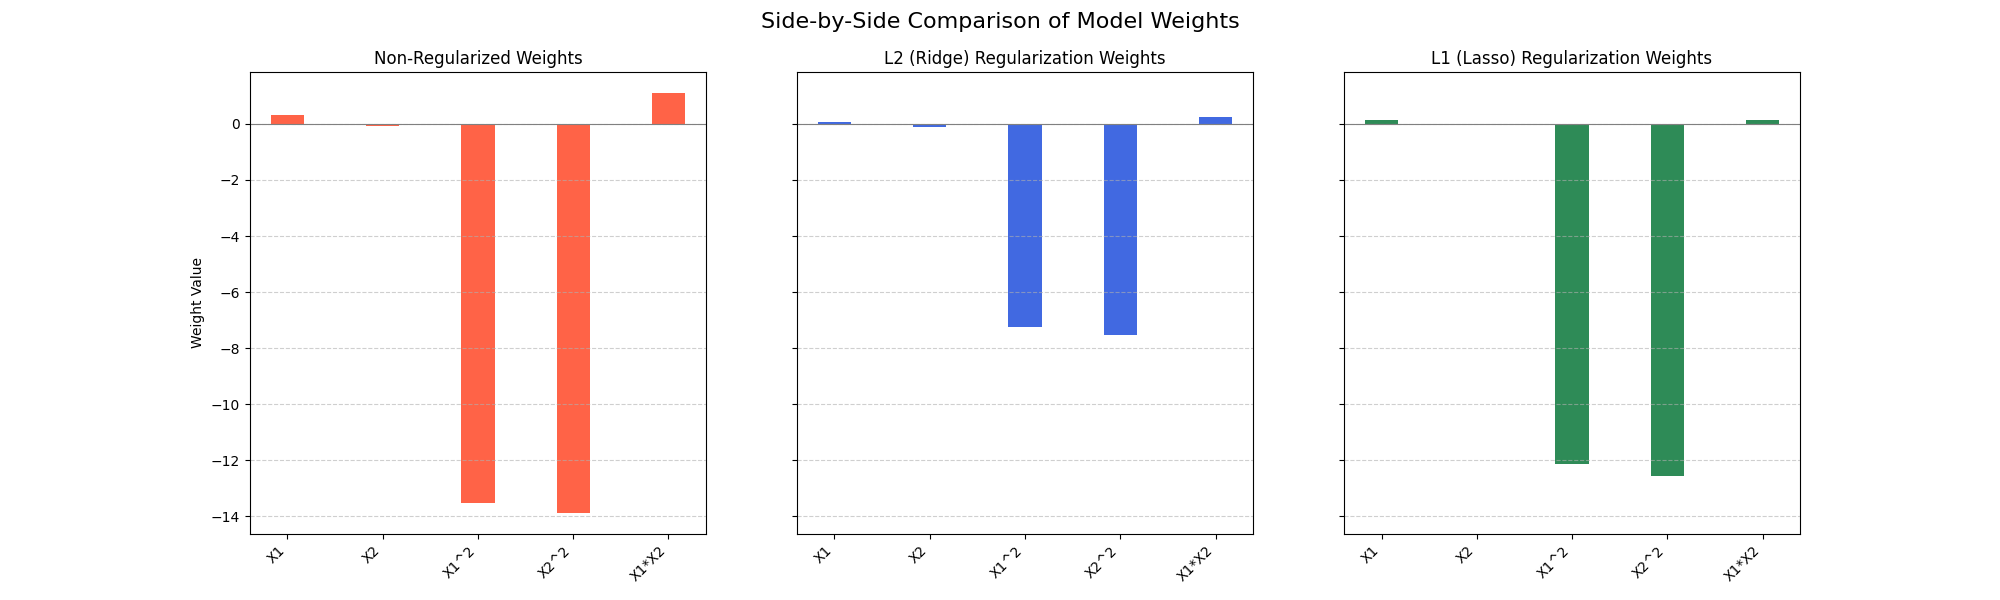
\includegraphics[width=1\linewidth]{submission_4b.png} \\
				      \textbf{Figure 3: Comparision of Regularization Methods}
			      \end{center}
			\item ii. Best Performing Hyperparameter Combination (shown in Figure 4): \\
			      --- Grid Search Results --- \\
			      Best parameters found: \{'learning\_rate': 0.1, 'lambda\_val': 0.0001\} \\
			      Best validation accuracy: 100.00\% \\
			      Test Set Accuracy: 98.67\% \\

			      \begin{center}
				      \centering
				      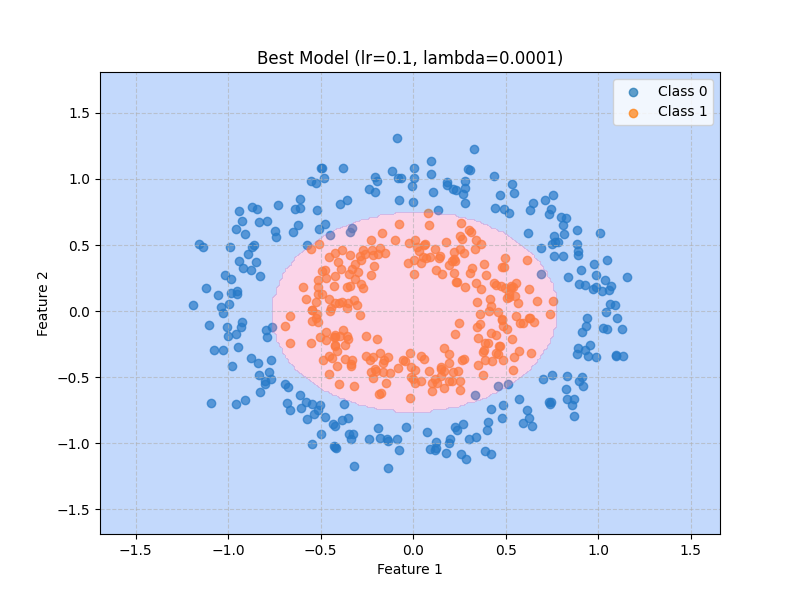
\includegraphics[width=1\linewidth]{submission_4c.png} \\
				      \textbf{Figure 4: Best Performing Hyperparameter Combination}
			      \end{center}

			\item ii. As shown in Figure 5, Stochastic GD converges the fastest while Batch GD provide the most stable and predictable convergence. Since the plot displays the result averaged by epochs, it is unable to see the oscillating individual updates of Mini-batch GD and Stochastic GD.
			      Based on this plot, we can conclude that in terms of convergence speed: Stochastic GD \textgreater Mini-batch GD \textgreater Batch GD, as they make increasingly more parameter updates per epoch. However, in terms of stability of convergence: Batch GD \textgreater Mini-batch GD \textgreater Stochastic GD.

			      \begin{center}
				      \centering
				      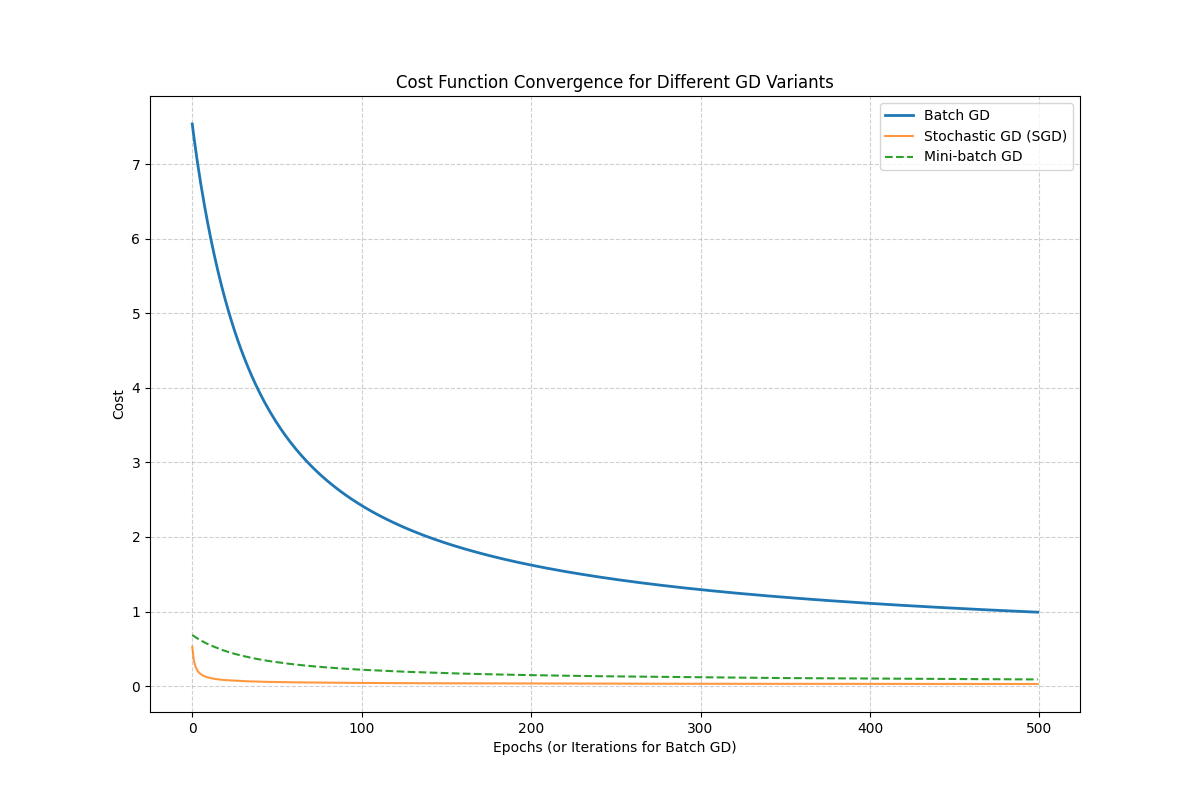
\includegraphics[width=1\linewidth]{submission_4d.png} \\
				      \textbf{Figure 5: Comparision of Different GD Variants}
			      \end{center}

		\end{enumerate}

	\end{tcolorbox}
\end{enumerate}

\end{document}
